
\begin{figure}[ht]
  \centering
  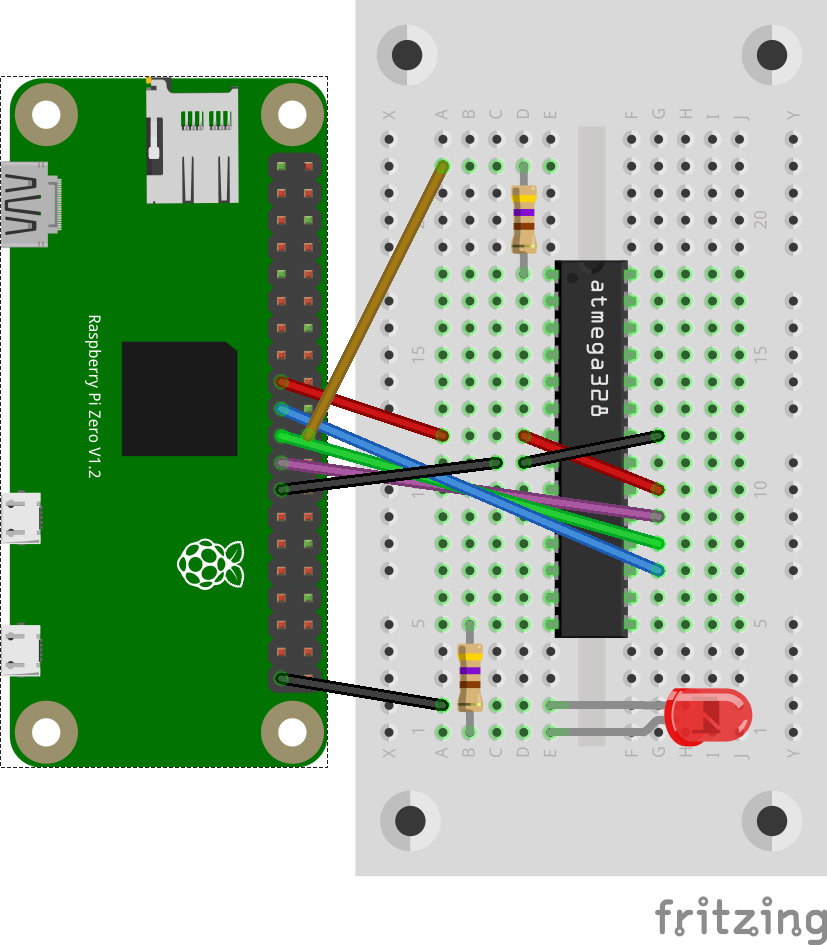
\includegraphics[scale=0.19]{images/ATmega328P_Steckplatine.png}	
  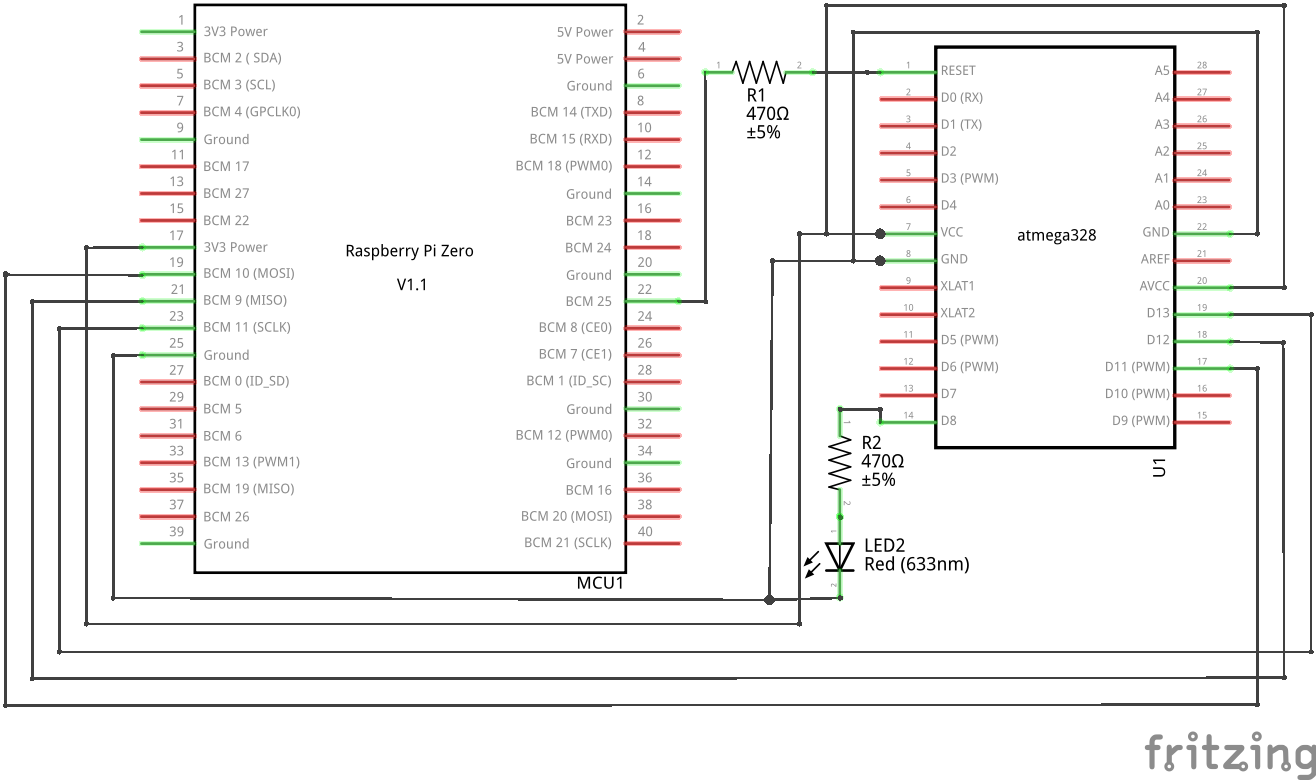
\includegraphics[scale=0.19]{images/ATmega328P_Schaltplan.png}	
  % \caption{}
  \label{ATmega328P}
\end{figure}

\subsection{Einrichtung}

Bei Raspjamming-Image wurde die Einrichtung bereits vorgenommen. Die folgenden Schritte sind also nur n�tig wenn die Installation auf einem anderen System erfolgt.

\begin{console}
sudo apt-get install avrdude
\end{console}

In der Konfigurationsdatei /etc/avrdude.conf muss die SPI-Taktfrequenz von 400~kHz auf 200~kHz reduziert werden.

\begin{screensmall}
  id = "linuxspi";
  desc = "Use Linux SPI device in /dev/spidev*";
  type = "linuxspi";
  reset = 25;
  baudrate=200000;
\end{screensmall}

\subsection{Verbindungstest}

Mit "`avrdude"' kann der Chiptyp ausgelesen bzw. die Kommunikation gepr�ft werden. Bei GC2-xHAT muss allerdings der Befehl "`atpoweron"' zuerst ausgef�hrt werden.
\begin{console}
sudo avrdude -c linuxspi -p m328p -P /dev/spidev0.0
\end{console}

\begin{screensmall}
avrdude: AVR device initialized and ready to accept instructions
Reading | ################################################## | 100% 0.00s
avrdude: Device signature = 0x1e950f (probably m328p)
avrdude: safemode: Fuses OK (E:FF, H:D9, L:62)
avrdude done.  Thank you.
\end{screensmall}

\subsection{Programmierung}

\begin{console}
sudo apt-get install gcc-avr avr-libc 
\end{console}

Zum Programmieren, Kompilieren und �bertragen einen Programms in den ATmega328P siehe \url{https://blog.gc2.at/post/atmega-328p/}